The Mars Rover is a Sample Return Rover designed by the JPL NASA Laboratory. It consists of a chassis with a central revolute joint on both the left and right sides of the robot. The central revolute joint is connected to two links (on each side),  for the front and rear wheels. Each respective link is connected to another link downward that is connected to a wheel. The front links are revolute so that the robot can turn left and right.

Primitive designs of this robot had a large amount of damage to the rover’s wheels. This wheel damage reduced the longevity of the Mars Rover mission by a great amount. NASA had to counteract this damage through researching the cause of the wheel damage. The rover did not properly avoid terrain obstacles nor did it deal with traction loss. The goal for this project is to recreate the traction control algorithm and simulate the results. The algorithm for the traction control is a velocity-based algorithm. One wheel on the rover will be rotating much faster than the others. The traction control system then applies a brake to that wheel to reduce its slip and then reducing wheel slip.


%Here is some example text, which lives in the file \textit{srr\textunderscore ws/src/srr/latex/ traction\textunderscore control/sections/introduction/introduction.tex}, and is made an input in \textit{srr\textunderscore ws/src/srr/latex/traction\textunderscore control/traction\textunderscore control.tex}. LaTeX uses a bunch of macros to stylize and simplify writing reports like these, like how the filepaths were italicized with the \textbf{\textbackslash textit} command. There's a text environment, where this text is being written in, and then there's a math environment, which can format stuff to be all pretty such as:
%
%\begin{equation}\label{traction_control:intro:quad}
%	x_{1,2} = \frac{-b \pm \sqrt{b^{2} - 4ac}}{2a}
%\end{equation}
%
%And then you can reference the super important equation \eqref{traction_control:intro:quad} by naming it, so you never have to keep track of which number equation it is, etc. \\
%
%Ending a line with \text{\textbackslash \textbackslash} will force a new line, like just above this sentence. Also, here's a figure with a centered caption below it:
%
%\begin{figure}[htbp]
%	\centering
%	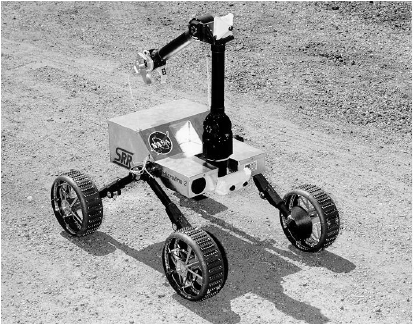
\includegraphics[width=.9\textwidth]{sections/introduction/images/srr.png}
%	\caption{An Early Version of the Sample-Return Rover}
%\end{figure}
%
%Again, it's numbered automatically, so we don't have to change that if we decide to move stuff around. If we decide to change the style later, we just have to renew commands and recompile, we don't have to change the content of these files, etc. There are even likely premade IEEE stylesheets that can be imported and automatically applied to everything in this document. \\
%
%Press the green button at the top to compile the main .tex file, TeXstudio will render a preview of the document for you. You can right click on the PDF preview and click "Go to Source" if you want to open the location of whatever it is you clicked on, if you see a typo you want to change quickly, etc. Try it with this paragraph or the figure.
